% Figure 1 (architecture) source. No data dependency beyond code facts in
% data/values.tex. Compile from paper/ with:
%   pdflatex -output-directory=figures-static figures-src/fig-architecture.tex
% The PDF is included by sections/03-architecture.tex in both manuscript builds
% (TikZ cannot be loaded together with ieeeaccess.cls).
\documentclass[border=1pt]{standalone}
\usepackage[T1]{fontenc}
\usepackage{mathptmx}
\usepackage{tikz}
\usetikzlibrary{arrows.meta,positioning,fit}
\input{data/values.tex}
\begin{document}
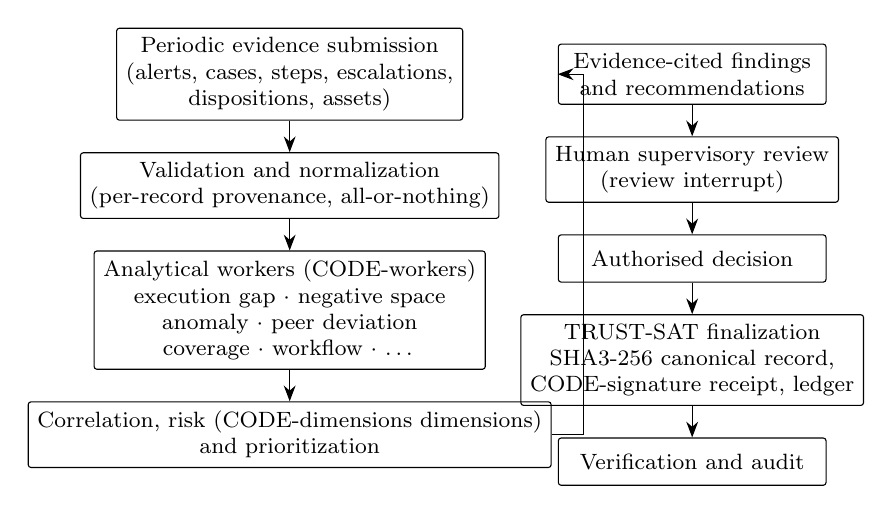
\begin{tikzpicture}[node distance=4mm and 6mm, every node/.style={font=\footnotesize},
  box/.style={draw, rounded corners=1pt, align=center, minimum width=34mm, minimum height=6mm},
  arr/.style={-{Stealth[length=2mm]}}]
\node[box] (sub) {Periodic evidence submission\\(alerts, cases, steps, escalations,\\dispositions, assets)};
\node[box, below=of sub] (val) {Validation and normalization\\(per-record provenance, all-or-nothing)};
\node[box, below=of val, minimum height=14mm] (ana) {Analytical workers (\V{CODE-workers})\\execution gap $\cdot$ negative space\\anomaly $\cdot$ peer deviation\\coverage $\cdot$ workflow $\cdot$ \ldots};
\node[box, below=of ana] (risk) {Correlation, risk (\V{CODE-dimensions} dimensions)\\and prioritization};
\node[box, right=12mm of sub] (find) {Evidence-cited findings\\and recommendations};
\node[box, below=of find] (rev) {Human supervisory review\\(review interrupt)};
\node[box, below=of rev] (dec) {Authorised decision};
\node[box, below=of dec] (trust) {TRUST-SAT finalization\\SHA3-256 canonical record,\\\V{CODE-signature} receipt, ledger};
\node[box, below=of trust] (ver) {Verification and audit};
\draw[arr] (sub) -- (val); \draw[arr] (val) -- (ana); \draw[arr] (ana) -- (risk);
\draw[arr] (risk.east) -| ++(4mm,0) |- (find.west);
\draw[arr] (find) -- (rev); \draw[arr] (rev) -- (dec); \draw[arr] (dec) -- (trust); \draw[arr] (trust) -- (ver);
\end{tikzpicture}
\end{document}
